\section{Greedy Algorithms}

  Greedy algorithms are easy to implement and easy to conceptualize, but they are often not correct. So the only interest in them is proving if they are correct. We have done greedy algorithms like Dijkstra and finding MSTs. Every step, greedy algorithms make an irrevocable decision of what to do and cannot undo it. That is, we cannot backtrack. In fact, some algorithms like Kruskal's algorithm for MSTs is precisely a greedy algorithm. 
  
  \begin{example}[Interval Scheduling]
    Let there be 1 classroom and $n$ courses, each with a start and end time $(s_i, e_i)$. We want to find the largest subset of courses that can be scheduled in a day such that they don't overlap. There are two things we want to do. How do we code this up? How do we show that a greedy algorithm will give a correct answer? Two greedy approaches are as follows. 
    \begin{enumerate}
      \item Sort them by the start times, and add them as long as they do not overlap with what you have. This will not work. 
      \item Sort them by the time interval lengths and keep adding them as long as they do not overlap with what you have. This will not work either. 
    \end{enumerate}
    It turns out that if we sort based on finish time, this will work. So why is this correct? Assume that the first $k$ decisions of this greedy algorithm are correct. Then, to find the next interval that we will include, the optimal algorithm must choose one that does not overlap with what we have. This is good since we do the same. The second part is that the next added interval must have the smallest end time $t$ from all viable left intervals. Assume that it was not and that the optimal next interval had end time $s > t$. Then, the next interval must start after $s$, but this also starts after $t$, so we are sacrificing unnecessary extra space. An optimal solution with the endpoint at $s$ can also be constructed with the same interval ending at $t$ without anything to lose. 

    \begin{algorithm}[H]
      \caption{Find Max Classes to Fit into 1 Room}
      \label{alg:class1}
      \begin{algorithmic}
        \Require{classes $C = \{(s_i, e_i)\}_i$ of type \texttt{List[tuple(int, int)]}}
        \Function{Schedule}{\texttt{C}}
          \State $\texttt{res} \gets \texttt{[]}$ 
          \State sort $C$ by increasing end time
          \For{$s, e \in C$} 
            \If{$s < \texttt{res[-1][-1]}$} \Comment{If start overlaps with previous end time}
              \State continue
            \EndIf
            \State add $(s, e)$ to res \Comment{Otherwise add class to final schedule}
          \EndFor
          \State \Return{\texttt{res}}
        \EndFunction
      \end{algorithmic}
    \end{algorithm}
    To get the run time, the sorting takes $O(n \log{n})$ time and iterating is $O(n)$, so a total of $O(n \log{n})$ time. 
  \end{example}

  \begin{example}[Classroom Scheduling]
    A slightly more practical example is that you have $n$ classes and you want to minimize the number of classrooms $m$. For this, you can really use any order. The general idea is 
    \begin{enumerate}
      \item Consider intervals in increasing start time $s_i$. 
      \item If it can be scheduled in an existing classroom, then schedule it there. 
      \item If not, then open a new classroom. 
    \end{enumerate}
    Even then, we can conduct a line search through all the time periods, incrementing the current number of classes if an incoming time is a start time and decrementing if it is an end time. We report the max $\Delta$ over all times. 

    This algorithm is correct since by definition, $\Delta$ is the lower bound for the number of classrooms needed and the greedy algorithm attains it. The greedy algorithm reports $\Delta$ since if it reported $\Delta +1$ classroom, then at some time $t$ it opened the $\Delta+1$th classroom. But this is impossible since this must mean that there are $\Delta + 1$ classrooms concurrently in use, contradicting our assumption that $\Delta$ is the optimal solution. 

    \begin{algorithm}[H]
      \caption{Minimizing Number of Rooms With $n$ Classes (Leetcode 253, Meeting Rooms II)}
      \label{alg:class_schedule}
      \begin{algorithmic}
        \Require{classes $C = \{(s_i, e_i)\}_i$ of type \texttt{List[tuple(int, int)]}}
        \Function{MeetingRooms}{$C$} 
          \State $\texttt{start} \gets$ all start times sorted increasing 
          \State $\texttt{end} \gets$ all end times sorted increasing 
          \State $\texttt{res} \gets 0$ \Comment{Our max classes count} 
          \State $\texttt{count} \gets 0$ \Comment{Our curr. classes count} 
          \State $\texttt{s}, \texttt{e} \gets 0$ \Comment{pointers for \texttt{start}, \texttt{end}} 

          \While{\texttt{s < len(start)}} \Comment{Don't need to check for \texttt{end} since}
            \If{\texttt{start[s] == \texttt{end[e]}}} \Comment{\texttt{start} will always finish faster.}
              \State \texttt{s += 1, e += 1} \Comment{One started and one ended, so don't change}
            \ElsIf{\texttt{start[s] > \texttt{end[e]}}} 
              \State \texttt{e += 1, count -= 1} \Comment{One ended, so decrement \texttt{count}}
            \ElsIf{\texttt{start[s] < \texttt{end[e]}}}
              \State \texttt{s += 1, count += 1} \Comment{One started, so increment \texttt{count}}
              \State \texttt{res = max(res, count)} \Comment{Update res if we got past it}
            \EndIf
          \EndWhile

          \State \Return{res}
        \EndFunction
      \end{algorithmic}
    \end{algorithm}

    The runtime is $O(n \log{n})$, which is to sort. However, you don't even need to sort since you can go through all intervals in any order and place it in an existing classroom or open a new classroom. 
  \end{example}

  The next one isn't as trivial, but requires us to devise a custom sorting method by comparing two sequences with a swap difference. 

  \begin{example}[Quiz Problem]
    Suppose you have $n$ questions with question $i$ having reward $r_i$, but the probability that you get it correct is $p_i$. You keep collecting the reward until you get one question wrong, and the game terminates. What order would you answer the questions in? 

    Suppose we have $q = (10, 5)$ and $r = (0.1, 0.2)$. 
    \begin{enumerate}
      \item If you choose the first and then second, then the expected return is 
        \begin{equation}
          10 \cdot 0.1 + 5 \cdot 0.1 \cdot 0.2 = 1.1 
        \end{equation}

      \item If you choose the second and then first, then the expected return is 
        \begin{equation}
          5 \cdot 0.2 + 10 \cdot 0.1 \cdot 0.2 = 1.2
        \end{equation}
    \end{enumerate}
    Clearly, finding all possibilities is too computationally expensive since it increases exponentially w.r.t. $n$. Intuitively, if I have a question with a high reward, I want to answer it first, but if I have a low probability of getting it correctly, then I can't answer future questions if I get it wrong. So I have to balance these two forces. So we want to sort the score of each question with some function $f(r_i, p_i)$, which is increasing in both $r_i$ and $p_i$. It is not $r_i p_i$, but this is a good start. 
    
    Rather, we can take a different approach. Assume that the tuples were sorted in some order, but this was not the optimal order. Then this indicates that we can swap to adjacent elements and it will get a better order. This is really like bubble sort, and now we need to find out the conditions on which it can be improved.  
    \begin{enumerate}
      \item If we answer $q_1 \rightarrow q_2 \rightarrow q_3 \ldots$, our expected reward is 
        \begin{equation}
          \mathbb{E}[R] = r_1 p_1 + r_2 p_1 p_2 + r_3 p_1 p_2 p_3 
        \end{equation}
      \item If we swap $q_2$ and $q_3$ and answer $q_1 \rightarrow q_3 \rightarrow q_2 \ldots$, then our expected reward is 
        \begin{equation}
          \mathbb{E}[R] = r_1 p_1 + r_3 p_1 p_3 + r_2 p_1 p_2 p_3 
        \end{equation}
      Note that the swap does not affect higher order terms. Doing some algebra, the swap is better iff 
      \begin{equation}
        r_2 p_2 (1 - p_3) < r_3 p_3 (1 - p_2) \implies \frac{r_2 p_2}{1 - p_2} < \frac{r_3 p_3}{1 - p_3}
      \end{equation}
      where the final swap saves computational time since we can compute for a single element rather than comparing pairwise elements. So, we sort it (in descending order!) according to these values to maximize this value. Note that the numerator measures your expected reward, while the denominator measures the probability of you screwing up. 

    \end{enumerate}
  \end{example}

  Not all greedy problems admit to scoring functions however. This was just one example. 

  \begin{example}[Minimizing Max Lateness]
    Suppose there are $n$ jobs that all come in at once at time $0$, with job $j$ having length $p_j$ and deadline $d_j$. We want to schedule the order of jobs on one machine that can handle one job at a time, where you must minimize the maximum lateness, where the lateness of job $i$ is $\max\{f_i - d_i, 0\} = [f_i - d_i]^+$. 

    For example, given jobs $(p, d) = \{(10, 9), (8, 11)\}$, we can run it in two ways. 
    \begin{enumerate}
      \item Running 1 then 2. The first job finishes at $10$ and the second at $18$. The lateness is $10 - 9 = 1$ and $18 - 11 = 7$ respectively, so the maximum lateness is $7$. 
      \item Running 2 then 1. The first job finishes at $8$ and the second at $18$. The lateness is $0$ and $18 - 9 = 9$, so the maximum lateness is $9$.  
    \end{enumerate}
    Therefore, $1 \rightarrow 2$ beats $2 \rightarrow 1$. Clearly, brute forcing this over $N!$ jobs orderings is unfeasible, but there is a greedy approach to this. We can 
    \begin{enumerate}
      \item schedule jobs in increasing order of deadlines. 
      \item try to exchange by taking a sequence, swapping it, and computing the score like we did for previous examples. 
    \end{enumerate}
    Both lead to the same score/principle that we should schedule jobs in increasing order of deadlines. Let's prove this by taking jobs $i$ and $j$, where $d_j \leq d_i$. Then, if we schedule $i \rightarrow j$, then we have 
    \begin{align}
      l_i & = [t + p_i - d_i]^+ \\
      l_j & = [t + p_i + p_j - d_j]^+ 
    \end{align}
    with $l_j$ being the greatest late time. If we did $j \rightarrow i$, then we have 
    \begin{align}
      \hat{l}_j & = [t + p_j - d_j]^+ \\
      \hat{l}_i & = [t + p_i + p_j - d_i]^+ 
    \end{align}
    with $\hat{l}_i$ being the greatest late time. But this is a good sacrifice since we can see that both 
    \begin{equation}
      l_j > \hat{l}_j \text{ and } l_j > \hat{l}_i
    \end{equation}
    meaning that if we swap, then we will decrease the lateness of $j$ at the smaller cost of increasing that of $i$. Therefore, $j \rightarrow i$ is better. Note that even though the end times of the second job will always be the same between the two choices, starting with $j$ will give a later deadline time. So this means that in the optimal solution, we have to place them in this order of deadlines since we can always improve them by swapping. 
  \end{example}

  \begin{example}[Gift Wrapping a Convex Hull]
    Given $n$ points in $\mathbb{R}^2$, we want to find the subset of points on the boundary of its convex hull. We can intuit this by taking the bottom most point and imagine ``wrapping'' a string around the entire region.\footnote{This is called the gift wrapping algorithm.} Here's a basic fact. If we have a point $p_1 = (x_1, y_1)$ and we're looking at $p_2 = (x_2, y_2)$, and then $p_3 = (x_3, y_3)$ shows up, then we can look at the cross product 
    \begin{equation}
      P = (x_2 - x_1) (y_3 - y_1) - (y_2 - y_1)(x_3 - x_1) 
    \end{equation}
    and if $P > 0$, then $p_3$ is counterclockwise from $p_2$. The algorithm is as such. 
    \begin{enumerate}
      \item You choose the bottommost point and label it $p_1$. 
      \item You construct a vector pointing to the right and start turning it counterclockwise until it hits the first point. This can be done by iterating through all of the $n$ points and computing the angle. 
        \begin{equation}
          \tan{ \theta} = \frac{y_i - y_1}{x_i - x_1}
        \end{equation}
      and the points with the smallest such tangent value will be the desired point, which will be $\Theta(n)$. We set this point to be $p_2$ and claim that $p_1, p_2$ is in the convex hull. This is true since all point must lie above the line $p_1 p_2$. Now you do the same thing with $p_2$ starting with a vector facing to the right and rotating it left until it hits the first peg. Once you get to the topmost point, you can start the vector from the right and rotate it counterclockwise, but this is an implementation detail. 

      If your convex hull has $L$ vertices, then this algorithm will have $O(n L)$, which will be $O(n^2)$ worst case but if we sample uniformly, then we have $L \approx \log{n}$ and on average it is $O(n \log{n})$. 
    \end{enumerate}
    A lot of geometric algorithms is output sensitive. 
  \end{example}

  \begin{example}[Convex Hull with Graham Scan]
    In fact, we can take a different approach and get $O(n \log{n})$ time. 
    \begin{enumerate}
      \item You still start with $p_1$ with the minimum y-coordinate and we sort in increasing $\theta_i = \arctan \frac{y_i - y_1}{x_i - x_1}$. 
      \item Then it will walk from $p_i$ to $p_{i+1}$ and check at $p_{i+1}$ if it is on the convex hull or not. 
        \begin{enumerate}
          \item If you turned counterclockwise to go to $p_{i+1}$ then it's good and you're on the convex hull. 
          \item If you turned clockwise it is bad, and $p_i$ is not on the convex hull, so remove $p_i$. However, $p_{i-1}$ could also be clockwise as well, so you must backtrack and keep on removing points until you find a point $p_j$ such that the previous turn is counterclockwise. 
        \end{enumerate}
        Note that this is implemented as a stack. 
    \end{enumerate}
    This can be calculated in $O(1)$ by the previous cross product formula. 
    \begin{figure}[H]
      \centering 
      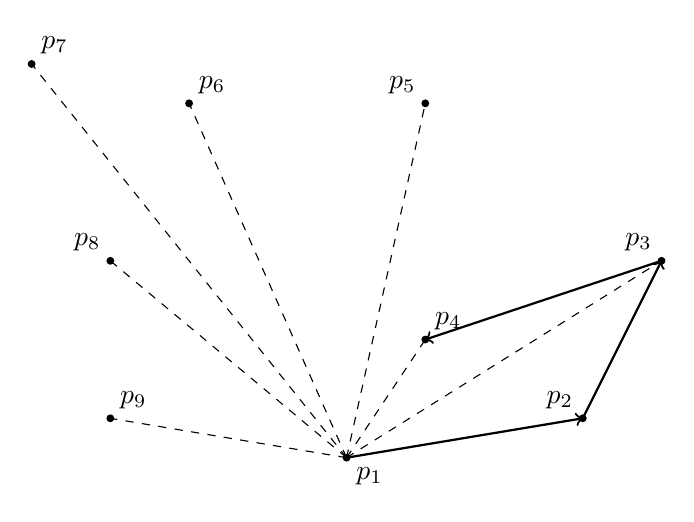
\begin{tikzpicture}
        \coordinate (p1) at (1,-2.5);  
        \coordinate (p7) at (-3,2.5);  
        \coordinate (p6) at (-1,2);  
        \coordinate (p4) at (2,-1);   
        \coordinate (p8) at (-2,0);  
        \coordinate (p5) at (2,2);   
        \coordinate (p3) at (5,0);   
        \coordinate (p9) at (-2,-2); 
        \coordinate (p2) at (4,-2);  
        
        % Draw dashed lines from p1 to all other points
        \draw[dashed] (p1) -- (p2);
        \draw[dashed] (p1) -- (p3);
        \draw[dashed] (p1) -- (p4);
        \draw[dashed] (p1) -- (p5);
        \draw[dashed] (p1) -- (p6);
        \draw[dashed] (p1) -- (p7);
        \draw[dashed] (p1) -- (p8);
        \draw[dashed] (p1) -- (p9);
        
        % Draw the points in black
        \fill[black] (p1) circle (0.05);
        \fill[black] (p2) circle (0.05);
        \fill[black] (p3) circle (0.05);
        \fill[black] (p4) circle (0.05);
        \fill[black] (p5) circle (0.05);
        \fill[black] (p6) circle (0.05);
        \fill[black] (p7) circle (0.05);
        \fill[black] (p8) circle (0.05);
        \fill[black] (p9) circle (0.05);

        \draw[->, thick] (p1) -- (p2);
        \draw[->, thick] (p2) -- (p3);
        \draw[->, thick] (p3) -- (p4);
        
        % Label the points (with small offset for readability)
        \node[below right] at (p1) {$p_1$};
        \node[above left] at (p2) {$p_2$};
        \node[above left] at (p3) {$p_3$};
        \node[above right] at (p4) {$p_4$};
        \node[above left] at (p5) {$p_5$};
        \node[above right] at (p6) {$p_6$};
        \node[above right] at (p7) {$p_7$};
        \node[above left] at (p8) {$p_8$};
        \node[above right] at (p9) {$p_9$};
      \end{tikzpicture}
      \caption{Visually, you start at the bottommost and rotate counterclockwise. } 
      \label{fig:graham}
    \end{figure}

    \begin{algorithm}[H]
      \caption{Finding Convex Hull with Graham Scan}
      \label{alg:graham}
      \begin{algorithmic}
        \Require{$p_1, \ldots, p_n \in \mathbb{R}^2$}
        \Function{Graham}{$\mathbf{p}$} 
          \State s $\gets$ stack()
          \State push $p_1, p_2$ onto s 
          \For{$i = 3, 4, \ldots, n$}
            \State push $p_i$ onto stack 
            \While{top 3 on stack are clockwise}
              \State pop second from top point 
            \EndWhile
          \EndFor 
          \State \Return{s} 
        \EndFunction
      \end{algorithmic}
    \end{algorithm}
    Note that once we have 3 points, the first three in the stack will always be counterclockwise, so we will never need to check if there are enough points in the stack. Even in the beginning, the next point (third) added is guaranteed to be counterclockwise because of ordering. Note that even though we might do a bunch of pushes and pops, the maximum number of pushes we can do is $n$ and pops is $n$, so this is $O(n)$. In fact, the bottleneck is the sorting, which is $O(n \log{n})$, so the total runtime is $O(n \log{n})$. 
  \end{example}

\subsection{Huffman Coding}

  Now, let's talk about \textbf{Huffman encoding}. We already know about the ASCII encoding that encodes characters in $7$ bits, for a total of $2^7$ possibilities. The extended ASCII uses $8$ bits, but all of these things use something called \textbf{fixed-length encoding} which uses a constant number of bits to encode any character. To compress something, we want to use \textbf{variable-length encoding}. 

  To decode something, the mapping from the characters to the bits must be injective, so we can define an inverse over its image. It turns out that if we an encoding for 3 characters, say 
  \[a \mapsto 1, b \mapsto 10, c \mapsto 11\]
  then decoding $1011$ is ambiguous since $1$ is a prefix of the encoding for $c$. Therefore, we do not want one encoding to be the prefix of another. It turns out that we can avoid this conflict by encoding everything as a binary tree and setting all encodings as leaf nodes. 

  \begin{figure}[H]
    \centering
    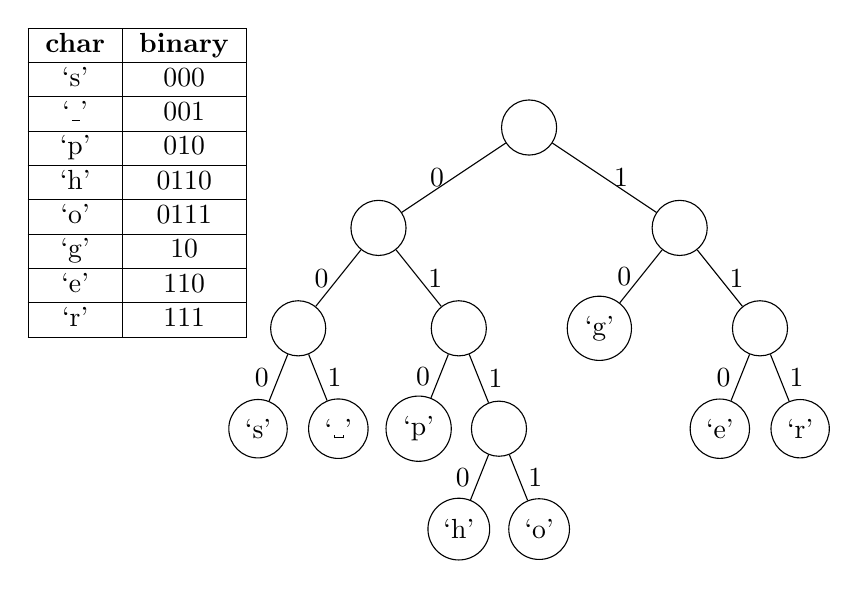
\begin{tikzpicture}[
      scale=0.85,
      level/.style={sibling distance=30mm/#1},
      level 1/.style={sibling distance=45mm},
      level 2/.style={sibling distance=24mm},
      level 3/.style={sibling distance=12mm},
      level 4/.style={sibling distance=12mm},
      inner/.style={circle, draw, minimum size=0.7cm},
      leaf/.style={circle, draw, minimum size=0.7cm},
      edge/.style={draw}
      ]
      
      % Create the tree structure
      \node[inner] {}
        child[edge from parent/.style={edge}] { node[inner] {}
          child[edge from parent/.style={edge}] { node[inner] {}
            child[edge from parent/.style={edge}] { node[leaf] {`s'} 
              edge from parent node[left] {0}
            }
            child[edge from parent/.style={edge}] { node[leaf] {`\textvisiblespace'} 
              edge from parent node[right] {1}
            }
            edge from parent node[left] {0}
          }
          child[edge from parent/.style={edge}] { node[inner] {}
            child[edge from parent/.style={edge}] { node[leaf] {`p'} 
              edge from parent node[left] {0}
            }
            child[edge from parent/.style={edge}] { node[inner] {} 
              child[edge from parent/.style={edge}] { node[inner] {`h'} 
                edge from parent node[left] {0}
              }
              child[edge from parent/.style={edge}] { node[inner] {`o'} 
                edge from parent node[right] {1}
              }
              edge from parent node[right] {1}
            }
            edge from parent node[right] {1}
          }
          edge from parent node[left] {0}
        }
        child[edge from parent/.style={edge}] { node[inner] {}
          child[edge from parent/.style={edge}] { node[leaf] {`g'} 
            edge from parent node[left] {0}
          }
          child[edge from parent/.style={edge}] { node[inner] {}
            child[edge from parent/.style={edge}] { node[leaf] {`e'} 
              edge from parent node[left] {0}
            }
            child[edge from parent/.style={edge}] { node[leaf] {`r'} 
              edge from parent node[right] {1}
            }
            edge from parent node[right] {1}
          }
          edge from parent node[right] {1}
        }
      ;
      
      % Create encoding table using minipage
      \node[anchor=north west, inner sep=0] at (-7.5,1.5) {
        \begin{minipage}{3.5cm}
          \begin{tabular}{|c|c|}
            \hline
            \textbf{char} & \textbf{binary} \\
            \hline
            `s' & 000 \\
            \hline
            `\_' & 001 \\
            \hline
            `p' & 010 \\
            \hline
            `h' & 0110 \\
            \hline
            `o' & 0111 \\
            \hline
            `g' & 10 \\
            \hline
            `e' & 110 \\
            \hline
            `r' & 111 \\
            \hline
          \end{tabular}
        \end{minipage}
      };
    \end{tikzpicture}
    \caption{Tree-based representation of prefix codes showing how different characters are encoded with variable-length binary sequences. The convention uses 0 for left branches and 1 for right branches. The encoding for each character is the sequence of 0's and 1's on the path from root to leaf. Characters are placed at leaf nodes to ensure the prefix property, with values deeper in the tree requiring more bits than those higher up.}
    \label{fig:prefix-tree}
  \end{figure}

  This makes sense since an encoding will be a prefix of another if and only if it is a parent of another. Furthermore, a greater depth of a character in the tree corresponds to a longer encoding. So, Huffman encoding tries to convert shorter characters to longer leaves and less recurrent characters into longer encodings. To decode a string of bits using a tree, we read the bit at a time to traverse left or right edge. When we reach a leaf, we decode the character and restart at root. 

  Now, we describe the greedy algorithm for building an optimal variable length encoding tree. 
  \begin{enumerate}
      \item We take the document and compute the frequencies of all characters that we want to encode. We want to less frequent characters to be lower on the tree, and so we will build the tree up from the leaves. 
      \item We iteratively choose the lowest weight nodes to connect up to a new node with weight = sum of children. 
  \end{enumerate}
  We implement this using a priority queue. 

  \begin{example}
    Let us go do an example of where we have the characters and frequencies 
    \begin{equation}
      a \mapsto 30, \; b \mapsto 20, \; c \mapsto 10, \; d \mapsto 15, \; e \mapsto 40
    \end{equation}

    \begin{figure}[H]
      \centering
      \begin{subfigure}[b]{0.48\textwidth}
      \centering
        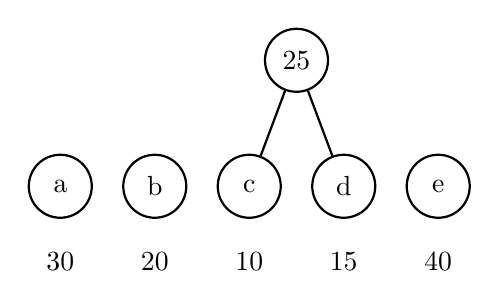
\begin{tikzpicture}[
            scale=0.8,
            node/.style={circle, draw, thick, minimum size=0.8cm},
            edge/.style={-,thick}
        ]
        % Vertices a through e at the bottom
        \node[node] (a) at (0,0) {a};
        \node[node] (b) at (1.5,0) {b};
        \node[node] (c) at (3,0) {c};
        \node[node] (d) at (4.5,0) {d};
        \node[node] (e) at (6,0) {e};
        % The vertex 25 at the top, positioned between c and d horizontally
        \node[node] (v5) at (3.75,2) {25};
        % Connect 25 to c and d
        \draw[edge] (v5) -- (c);
        \draw[edge] (v5) -- (d);
        % Add labels below the bottom vertices with increased spacing
        \node at (0,-1.2) {30};
        \node at (1.5,-1.2) {20};
        \node at (3,-1.2) {10};
        \node at (4.5,-1.2) {15};
        \node at (6,-1.2) {40};
        \end{tikzpicture}
        \caption{We write out them as leaf nodes with the values $30, 20, 10, 15, 40$. We take the smallest of the frequencies and sum them up: $10 + 15 = 25$.}
        \label{fig:step1}
      \end{subfigure}
      \hfill 
      \begin{subfigure}[b]{0.48\textwidth}
      \centering
        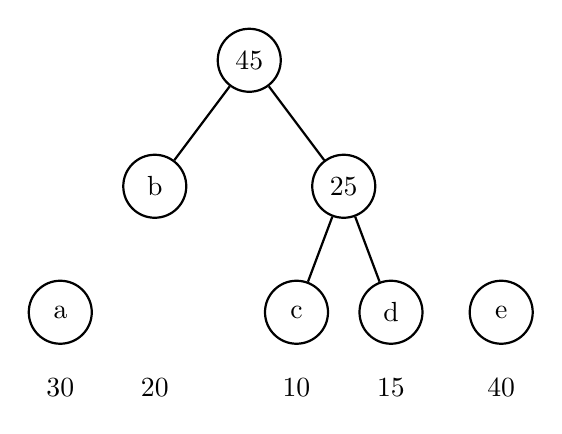
\begin{tikzpicture}[
            scale=0.8,
            node/.style={circle, draw, thick, minimum size=0.8cm},
            edge/.style={-,thick}
        ]
        % Top node (45)
        \node[node] (root) at (3,4) {45};
        % Second level nodes
        \node[node] (b) at (1.5,2) {b};
        \node[node] (v25) at (4.5,2) {25};
        % Bottom level connected nodes
        \node[node] (c) at (3.75,0) {c};
        \node[node] (d) at (5.25,0) {d};
        % Isolated nodes
        \node[node] (a) at (0,0) {a};
        \node[node] (e) at (7,0) {e};
        % Connections
        \draw[edge] (root) -- (b);
        \draw[edge] (root) -- (v25);
        \draw[edge] (v25) -- (c);
        \draw[edge] (v25) -- (d);
        % Add labels below the bottom vertices with good spacing
        \node at (0,-1.2) {30};
        \node at (1.5,-1.2) {20};
        \node at (3.75,-1.2) {10};
        \node at (5.25,-1.2) {15};
        \node at (7,-1.2) {40};
        \end{tikzpicture}
        \caption{We have the values $30, 20, 25, 40$. We sum the smallest two frequencies: $20 + 25 = 45$.}
        \label{fig:step2}
      \end{subfigure}
      
      \begin{subfigure}[b]{0.48\textwidth}
      \centering
        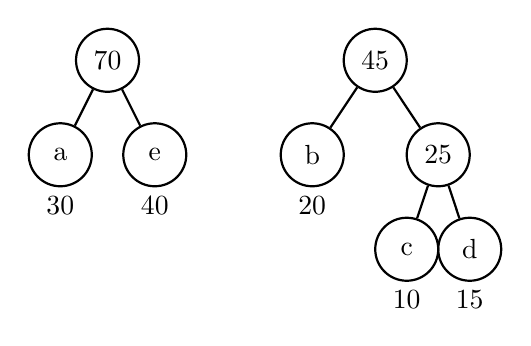
\begin{tikzpicture}[
            scale=0.8,
            node/.style={circle, draw, thick, minimum size=0.8cm}, % Smaller nodes
            edge/.style={-,thick}
        ]
        % Left tree - with reduced distances
        % Top node (70)
        \node[node] (left_root) at (-1.5,3) {70};
        % Bottom level for left tree
        \node[node] (a) at (-2.25,1.5) {a};
        \node[node] (e) at (-0.75,1.5) {e};
        % Connections for left tree
        \draw[edge] (left_root) -- (a);
        \draw[edge] (left_root) -- (e);
        % Add labels below the left tree nodes
        \node at (-2.25,0.7) {30};
        \node at (-0.75,0.7) {40};
        
        % Right tree - with reduced distances
        % Top node (45)
        \node[node] (right_root) at (2.75,3) {45};
        % Second level nodes for right tree
        \node[node] (b) at (1.75,1.5) {b};
        \node[node] (v25) at (3.75,1.5) {25};
        % Bottom level for right tree
        \node[node] (c) at (3.25,0) {c};
        \node[node] (d) at (4.25,0) {d};
        % Connections for right tree
        \draw[edge] (right_root) -- (b);
        \draw[edge] (right_root) -- (v25);
        \draw[edge] (v25) -- (c);
        \draw[edge] (v25) -- (d);
        % Add labels below the right tree nodes
        \node at (1.75,0.7) {20};
        \node at (3.25,-0.8) {10};
        \node at (4.25,-0.8) {15};
        \end{tikzpicture}
        \caption{We have the values $30, 45, 40$. We sum the smallest two frequencies: $30 + 40 = 70$.}
        \label{fig:step3}
      \end{subfigure}
      \hfill 
      \begin{subfigure}[b]{0.48\textwidth}
      \centering
        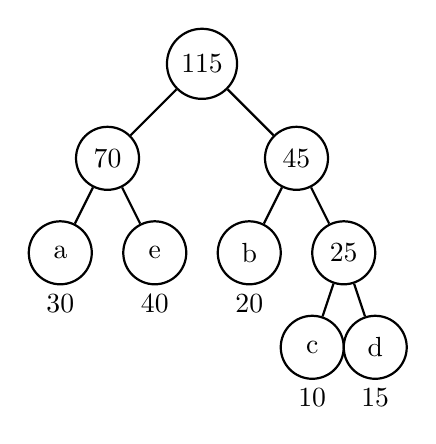
\begin{tikzpicture}[
            scale=0.8,
            node/.style={circle, draw, thick, minimum size=0.8cm}, % Smaller nodes
            edge/.style={-,thick}
        ]
        % More compact layout with reduced distances
        % Top node (115)
        \node[node] (root) at (2.25,4.5) {115};
        % Second level nodes
        \node[node] (v70) at (0.75,3) {70};
        \node[node] (v45) at (3.75,3) {45};
        % Connect top to second level
        \draw[edge] (root) -- (v70);
        \draw[edge] (root) -- (v45);
        % Third level nodes for left branch
        \node[node] (a) at (0,1.5) {a};
        \node[node] (e) at (1.5,1.5) {e};
        % Connect v70 to its children
        \draw[edge] (v70) -- (a);
        \draw[edge] (v70) -- (e);
        % Third level nodes for right branch
        \node[node] (b) at (3,1.5) {b};
        \node[node] (v25) at (4.5,1.5) {25};
        % Connect v45 to its children
        \draw[edge] (v45) -- (b);
        \draw[edge] (v45) -- (v25);
        % Fourth level nodes
        \node[node] (c) at (4,0) {c};
        \node[node] (d) at (5,0) {d};
        % Connect v25 to its children
        \draw[edge] (v25) -- (c);
        \draw[edge] (v25) -- (d);
        % Add labels below the bottom vertices
        \node at (0,0.7) {30};
        \node at (1.5,0.7) {40};
        \node at (3,0.7) {20};
        \node at (4,-0.8) {10};
        \node at (5,-0.8) {15};
        \end{tikzpicture}
        \caption{We have the values $70, 45$. We sum them up to get the complete tree.}
        \label{fig:step4}
      \end{subfigure}
      \caption{Building a Huffman encoding tree step by step}
      \label{fig:huffman-construction}
    \end{figure}
  \end{example}

  \begin{theorem}[Number of Nodes in Huffman Tree]
    If we have a document of $N$ total characters and $M$ unique characters, the number of nodes in the Huffman tree, in complexity notation, is 
    \begin{equation}
      O(M)
    \end{equation}
    Clearly, this has nothing to do with $N$. Note that we have $M$ leaf nodes, and in each iteration, we connect 2 nodes up to a parent. Therefore, the number of nodes to connect up decreases by 1 per iteration, and we create a new node per iteration. Since there are $M - 1$ iterations, we add one node, so there will be $M + M - 1 = O(n)$ nodes in the binary tree. 
  \end{theorem}

